\documentclass[11pt]{ctexart}
\usepackage[pdfborder=0 0 1]{hyperref}
\hypersetup{
    pdfauthor={Tsingpo Lee},
    pdftitle={长安大学 2017年招收攻读硕士研究生入学试题}, %文件标题
    pdfsubject={831,信号与系统,长安大学,考研}, %文件主题
    pdfcreator={The exam class (v \fileversion~as of \filedate)} % 应用程序
  }
\usepackage{geometry}
\usepackage{examanswersheet,caption2,pifont,ulem}
\usepackage{enumitem}
\definecolor{light-blue}{rgb}{0.8,0.85,1}
\pagecolor{black!17}
%\usepackage{draftwatermark}
%\SetWatermarkText{Made by Matthew}
%\SetWatermarkScale{1}
%\SetWatermarkLightness{0.75}
\usetikzlibrary{graphs}

\def\blob#1#2{\draw[blue,fill,rounded corners=#1*3mm] (#2) +($(0:#1*2+#1*rnd)$)
		\foreach \a in {20,40,...,350} {  -- +($(\a: #1*2+#1*rnd)$) } -- cycle;}
\usepackage{eso-pic}
\newcommand{\watermark}[3]{\AddToShipoutPictureBG{
\parbox[b][\paperheight]{\paperwidth}{
\vfill%
\centering%
\tikz[remember picture, overlay]%
  \node [rotate = #1, scale = #2] at (current page.center)%
    {#3};
\vfill}}}
\usepackage{enumerate,multicol,xcolor,fancyhdr,amsmath,tikz,pgf}
\mifengxian
\begin{document}
\watermark{10}{1}{\begin{tikzpicture}
	\blob{0.4}{8*rnd,13*rnd}
      \foreach \a in {0,20,...,550} {
		\fill[blue,opacity=rnd] let \p1 = (\a+20*rnd:3*rnd),
		\n1 = {0.2*rnd}
		in (\p1) circle(\n1);
	}
	
	\blob{0.2}{1*rnd,4*rnd}
	\foreach \a in {0,20,...,550} {
		\fill[blue,opacity=rnd] let \p1 = ($(1,3)+(\a+20*rnd:2*rnd)$),
		\n1 = {0.15*rnd}
		in (\p1) circle(\n1);
	}
	\end{tikzpicture}}

%
%	试卷标题
%
\begin{center}\bs{}
\zihao{3}{长安大学$2017$年招收攻读硕士研究生入学试题}\\
{\kaishu\zihao{5}{科目: 814信号与系统~~~~考试时间: 2016年12月25日}}
\end{center}
%
%	试卷正面
%
\begin{enumerate}[leftmargin=0em]
\vspace{3em}\setlength{\itemsep}{0em}
\item[\kaishu{}一]{\makebox[2mm][r]{、}\kaishu{}填空题(每空3 分,共30 分)}%--------------------------------------填空题
\item 已知序列$f(k)=\{1,2,3,4,5\}$,(首项序号$k=0$),求$f(k)=(k+3)\varepsilon(k)$的Z变换为\line{4}.\setlength{\itemsep}{3em}
\item 计算$\displaystyle\int_{0}^{10}t^2\delta(2t-2)\,{\rm d}t=$\line{4}.
\item 线性时不变系统输入$f(t)$与零状态响应$y(t)$之间的关系为$y(t)=\int_{-\infty}^{t}f(\tau-2)e^{-t-\tau}\,{\rm d}\tau$,求系统单位响应$h(t)=$\line{2}.
\item 利用能量等式$\displaystyle\int_{-\infty}^{\infty}f^2(t)\,{\rm d}t=\dfrac{1}{2\pi}\int_{-\infty}^{\infty}|F(j\omega)|^2\,{\rm d}\omega$,计算$\displaystyle\int_{-\infty}^{\infty}\left(\dfrac{\sin t}{t}\right)^2\,{\rm d}t=$\line{2}.
\item 信号$f(t)=4+5\cos \pi t+3\cos 2\pi t$的平均功率为\line{4}.
\item 已知$f(t)\leftrightarrow F(s)=\dfrac{3s+1}{s(s+1)}$,原函数的初值$f(0)=$\line{3}.
\item 已知某LTI某系统的激励为$f(t)=2^k\left[\varepsilon(k)-\varepsilon(k-3)\right]$,单位序列响应为$h(k)=\{\cdots,0,2,\underset{k=0}{\underset{\uparrow}{5}},3,0,\cdots\}$,则系统的零状态响应为\line{6}.
\item 已知信号$f(t)$的频谱函数$F(j\omega)=\begin{cases}
1,&|\omega|<2\,{\rm rad/s}\\
0,&|\omega|>2\,{\rm rad/s}
\end{cases}$,则对$f(3t)$进行理想采样的奈奎斯特采样间隔$T=$\line{2}.
\item 单边拉普拉斯变换$F(s)=\dfrac{e^{-(s+5)}}{s+5}$的原函数$f(t)$的原函数$f(t)=$\line{4}.
\item LTI离散系统的附中响应$g(k)=\left(\dfrac{1}{2}\right)^k\varepsilon(k)$,系统函数$H(z)=$\line{3}.
\vspace{3em}\setlength{\itemsep}{0em}
\item[\kaishu{}二]{\makebox[2mm][r]{、}\kaishu{}选择题(每小题3分,共30 分)}%-------------------------------------选择题
\item 某信号的频谱是周期的离散谱,则对应的时域信号为.
\setlength{\itemsep}{3em}
\xx{连续的周期信号}{连续的非周期信号}{离散的非周期信号}{离散的周期信号}
\item 以下等式不成立的是
\xxs{\int_{-\infty}^{\infty}f(\tau)\,{\rm d}\tau=f(t)*\varepsilon(t)}%
{\int_{-\infty}^{t}\delta(\tau)\,{\rm d}\tau=1}%
{f_1(t-t_0)*f_2(t+t_0)=f_1(t)*f_2(t)}%
{\delta(t)*f(t)*\delta(t)=f(t)}
\item 已知信号$f_1(t)$、$f_2(t)$如图1所示(a是常数),$f(t)=f_1(t)+f_2(t)$,则$f(t)$的傅里叶变换为
\xxs%
{\dfrac{a}{2}Sa\left(\dfrac{\omega a}{4}\right)+\dfrac{a}{2}Sa\left(\dfrac{\omega a}{2}\right)}%
{aSa\left(\dfrac{\omega a}{4}\right)+\dfrac{a}{2}Sa\left(\dfrac{\omega a}{2}\right)}%
{\dfrac{a}{2}Sa\left(\dfrac{\omega a}{4}\right)+aSa\left(\dfrac{\omega a}{2}\right)}%
{aSa\left(\dfrac{\omega a}{4}\right)+aSa\left(\dfrac{\omega a}{2}\right)}
\begin{center}
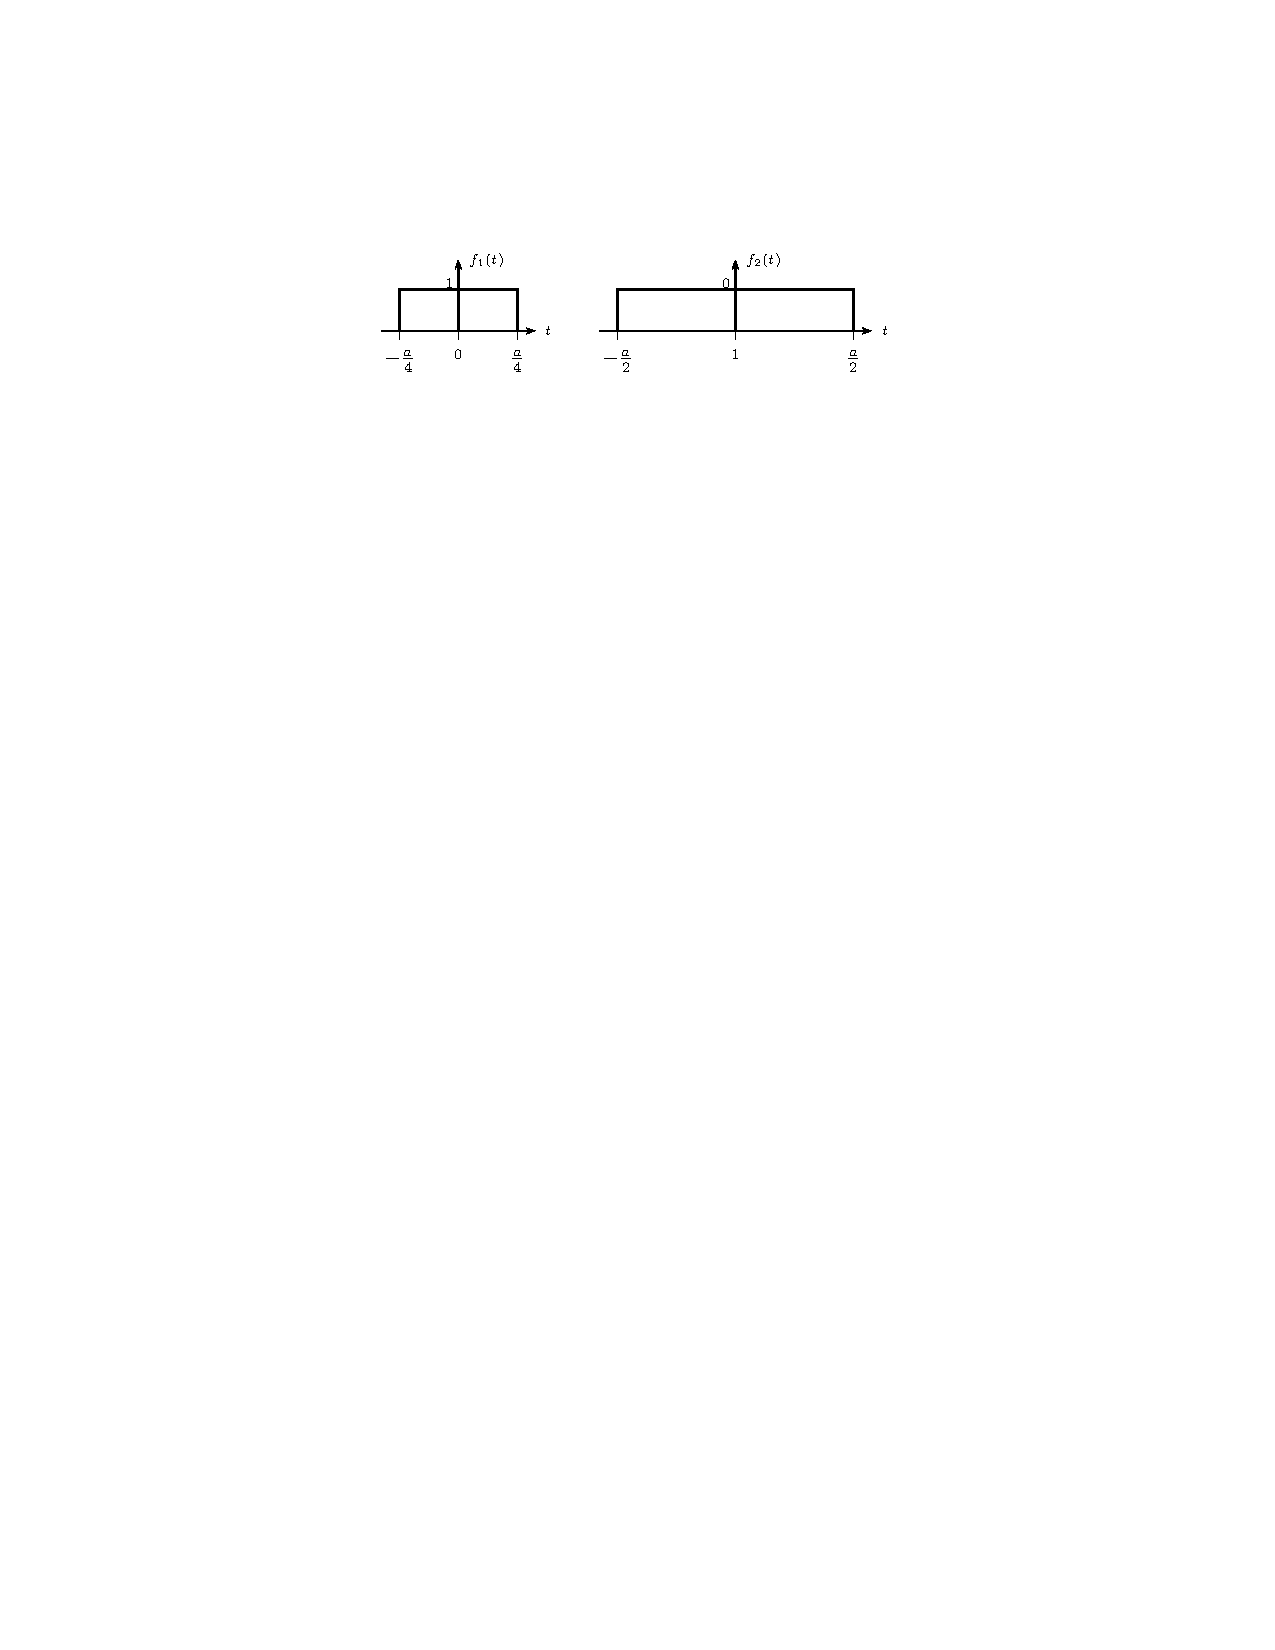
\includegraphics{img/14-2-1.pdf}\\
{\zihao{5}图1}
\end{center}
\item 下列信号中属于功率信号的是
\xxs%
{\cos t\varepsilon(t)}%
{e^{-t}\varepsilon(t)}%
{te^{-t}\varepsilon(t)}%
{e^{-|t|}}
\item 某系统的输出与输入关系满足$y'(t)+5y(t)=f(t+10)-2$,则该系统是
\xx%
{线性、时不变、因果}%
{线性、时变、因果}%
{非线性、时不变、非因果}%
{非线性、时变、非因果}
\item 序列$f(k)=\sin\left(\dfrac{\pi}{8}k\right)-3\cos\left(\dfrac{\pi}{4}k+\dfrac{\pi}{6}\right)+2\sin\left(\dfrac{\pi}{2}k-\dfrac{\pi}{4}\right)$的周期$N$为
\xxs{2}{4}{8}{16}

\item 已知系统微分方程为$y'(t)+2y(t)=2f(t)$,若$y(0_+)=\dfrac{4}{3}$,$f(t)=\varepsilon(t)$,解得全响应为$y(t)=\dfrac{1}{3}e^{-2t}+1,t\geqslant 0$,则全响应中$\dfrac{4}{3}e^{-2t}$为
\xx{零输入响应分量}{零状态响应分量}{自由响应分量}{强迫响应分量}
\item 设$f(t)\leftrightarrow F(j\omega)$,若$f_0(t)\leftrightarrow \dfrac{1}{4}F\left(j\dfrac{\omega}{4}\right)e^{j\frac{5}{4}\omega}$
\xxs{f(-4t+5)}%
{f(4t+5)}%
{f(-4t-5)}%
{f(4t-5)}
\newpage
\vspace{3em}
\newgeometry{a3paper,twocolumn,landscape,hmargin={1.3cm,3.5cm},vmargin={1.5cm,1.5cm},footskip=0.75cm,headsep=0.25cm}\savegeometry{back}
\item  已知某线性时不变系统,当输入信号$f(t)=(e^{-t}+e^{-3t})\varepsilon(t)$时,其零状态响应是$y(t)=(2e^{-t}-2e^{-4t})\varepsilon(t)$,则该系统的频率响应为
\xxs
{-\dfrac{3}{2}\left(\dfrac{1}{j\omega+4}+\dfrac{1}{j\omega+2}\right)}
{\dfrac{3}{2}\left(\dfrac{1}{j\omega+4}+\dfrac{1}{j\omega+2}\right)}
{\dfrac{3}{2}\left(\dfrac{1}{j\omega+4}-\dfrac{1}{j\omega+2}\right)}
{\dfrac{3}{2}\left(-\dfrac{1}{j\omega+4}+\dfrac{1}{j\omega+2}\right)}
\vspace*{3em}
\item 周期信号满足$f(t)=-f(-t)$时,则其傅里叶级数异形式中所含频率分量有
\xx{只有正弦项}{只有余弦项}{只有直流分量}{正弦余弦项都有}
\vspace{3em}\setlength{\itemsep}{0em}\setcounter{enumi}{0}
\item[\kaishu{}三]{\makebox[2mm][r]{、}\kaishu{}简答题(每小题5分, 共25 分)}%--
\item 简述拉普拉斯变换与傅里叶变换之间的关系,那么是否在斜体情况下函数的单边拉普拉斯变换存在,其傅里叶变换也存在呢?\setlength{\itemsep}{8em}
\item 其系统的频率响应$H(j\omega)=\dfrac{1+j\omega}{1-j\omega}$,试判断该系统是否为无失真传输系统?并说明理由。
\item 两个离散系统如图2a、图2b所示,请问两个离散系统是否等效?为什么?
\begin{center}
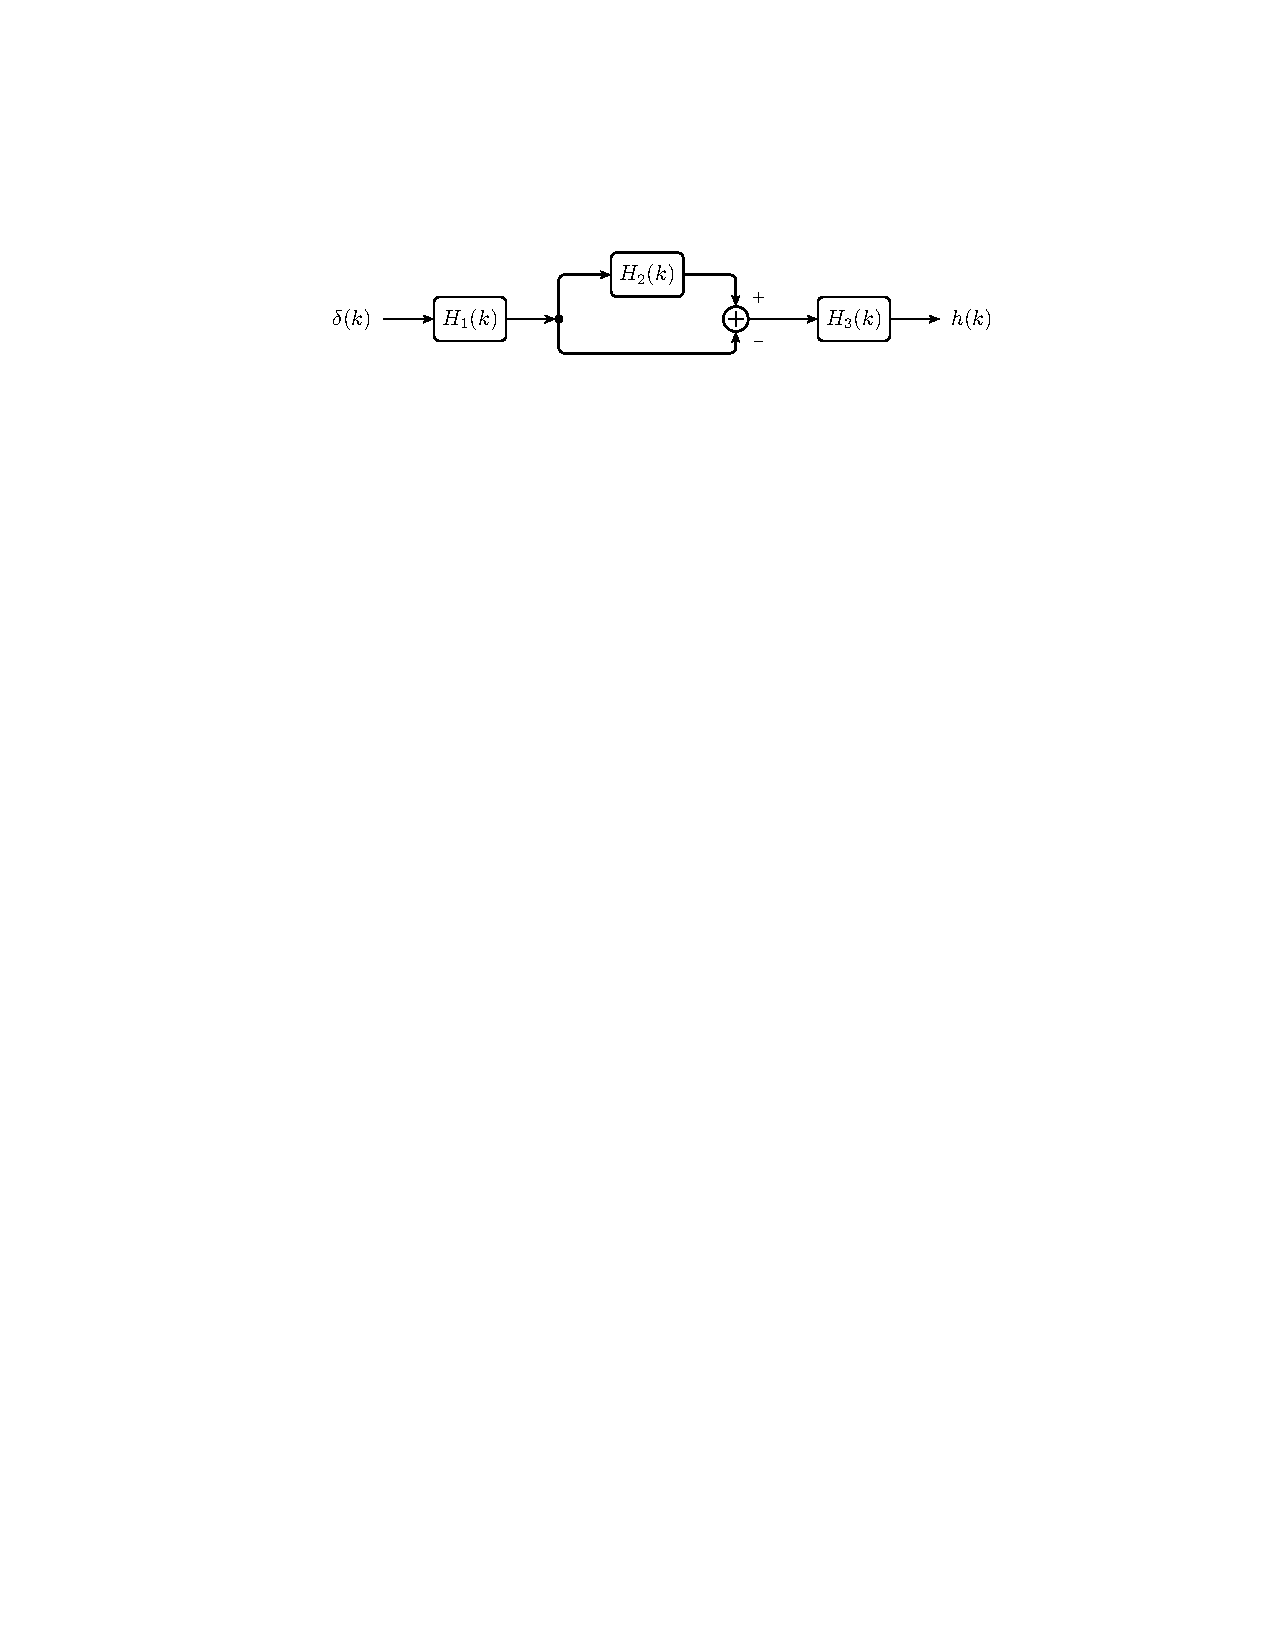
\includegraphics{img/6.pdf}\\
图2a\\
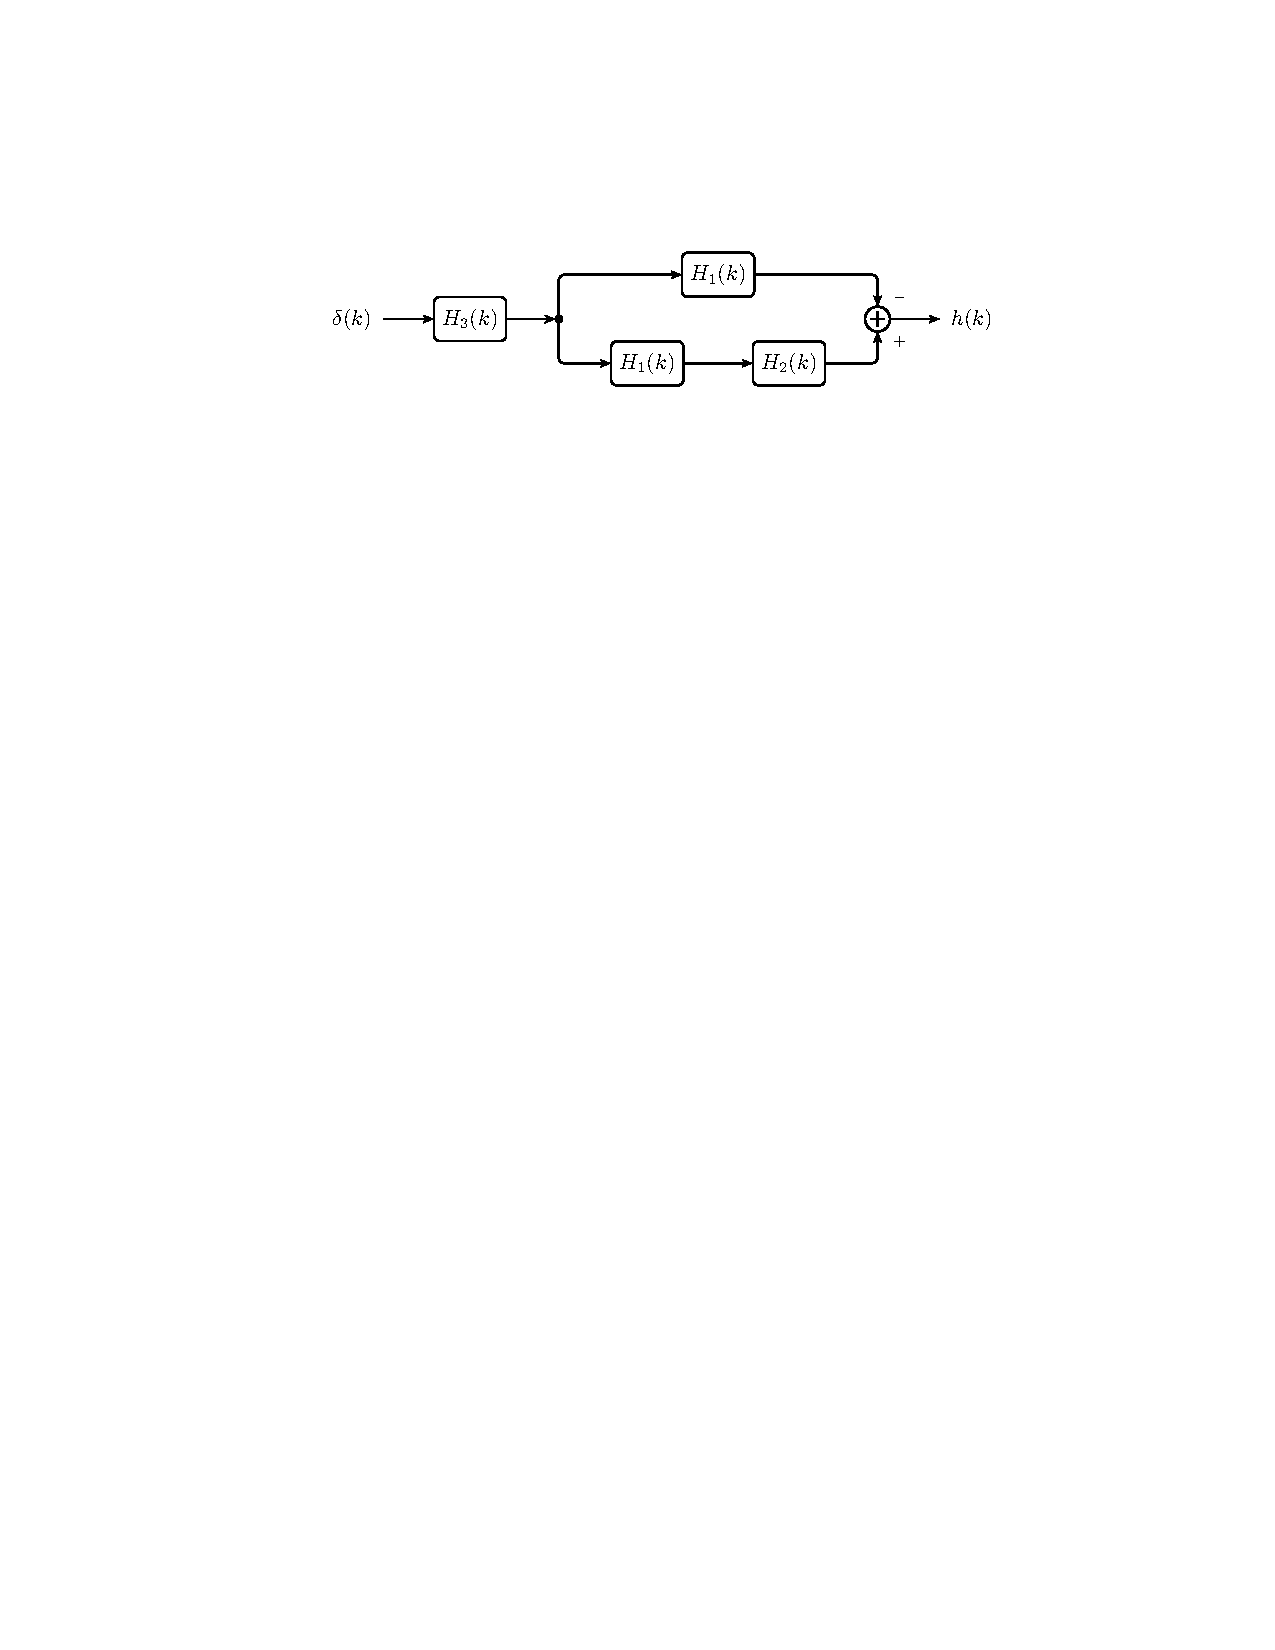
\includegraphics{img/7.pdf}\\
图2b
\end{center}
\item 试说明周期矩形脉冲当周期$T$不变、脉冲宽度$\tau$变小时,对谱线间隔和带宽的影响;当脉冲宽度$\tau$不变、周期$T$变大时,对谱线间隔和带宽的影响。
\item 简述什么是模拟信号、连续信号、离散信号和数字信号?
\setlength{\itemsep}{0em}\setcounter{enumi}{0}
\item[\kaishu{}四]{\makebox[2mm][r]{、}\kaishu{}计算综合题(65分)}%-----------------------------------------------计算题
\item (12分)已知信号$f(t)$的傅里叶变换为$F(j\omega)=|F(j\omega)|e^{j\varphi(\omega)}$,幅频特性如图3所示,相频特性$\varphi(\omega)=\omega$,试利用傅里叶变换的定义和性质计算:(不必求出$f(t)$)
\begin{center}
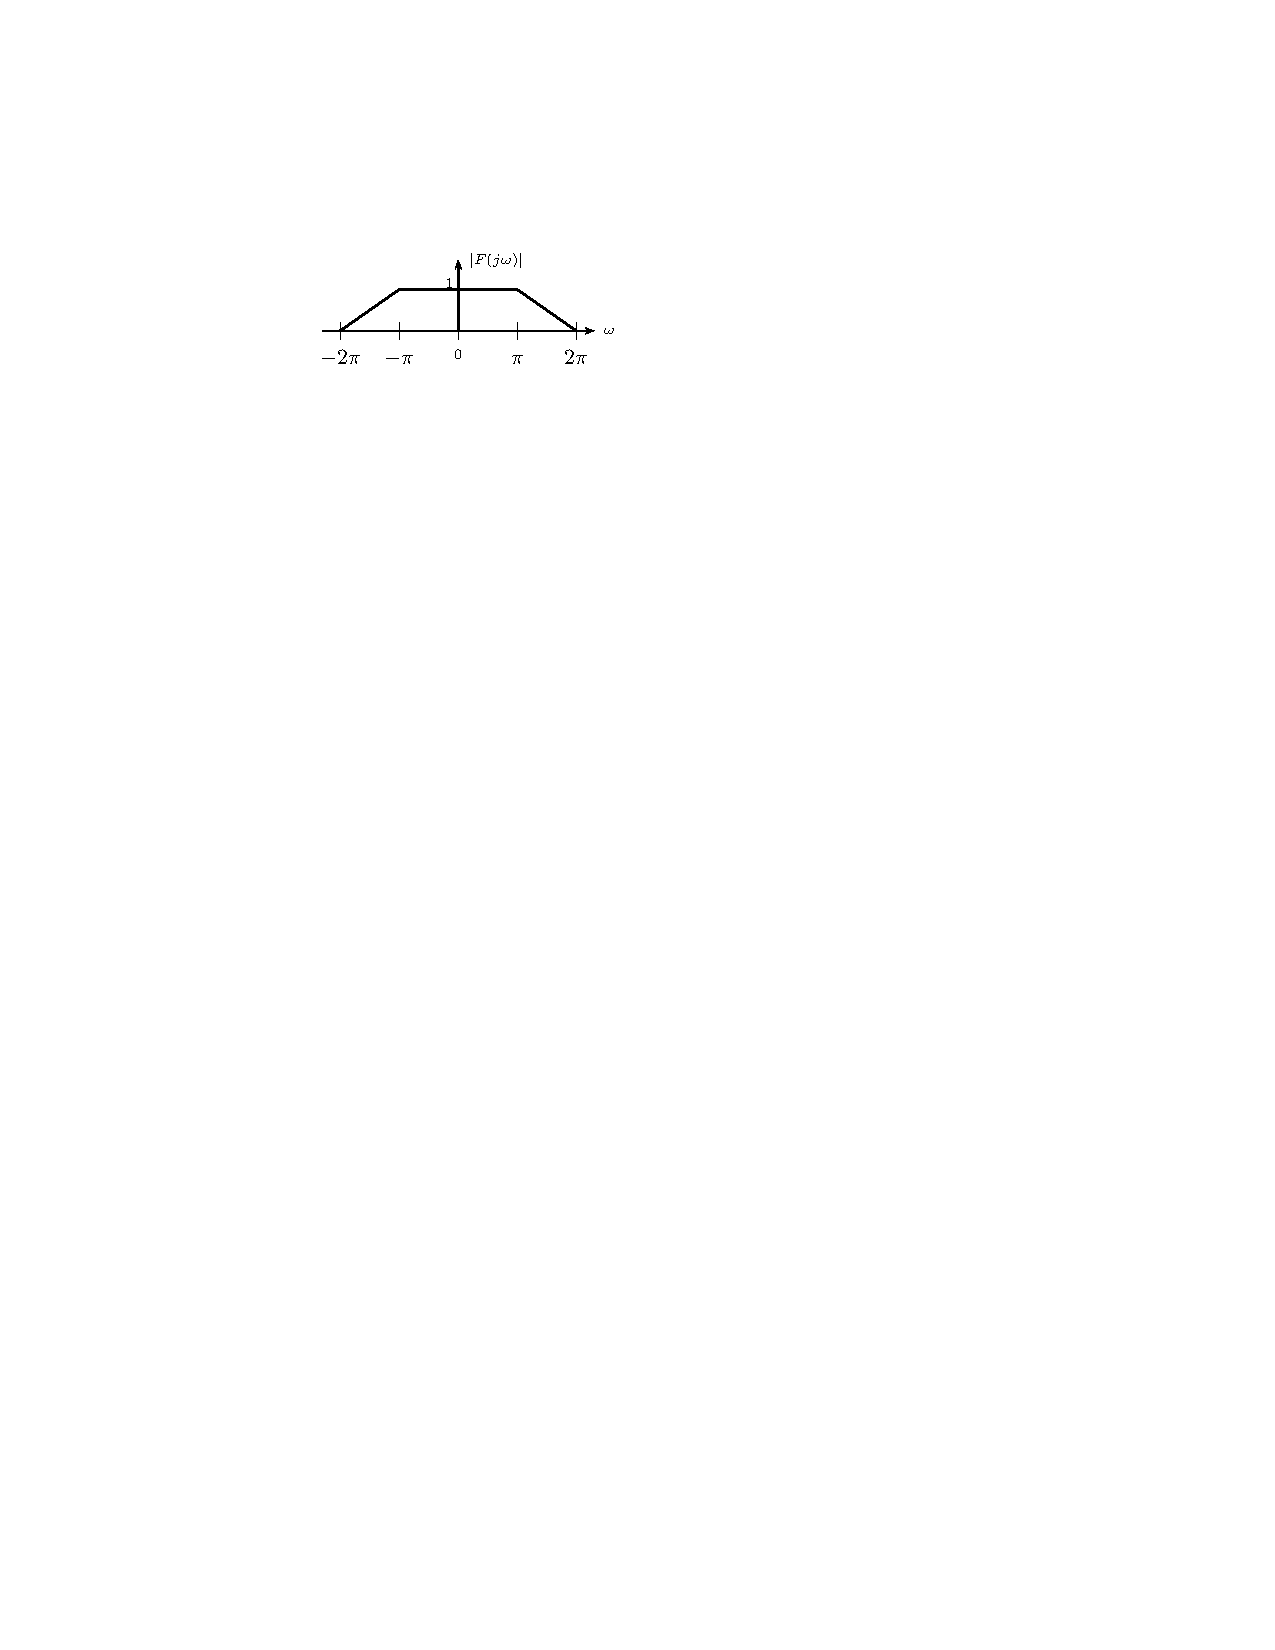
\includegraphics{img/14-2-2.pdf}\\
{\zihao{5}图3}
\end{center}
(1)$\displaystyle\int_{-\infty}^{+\infty}f(t)e^{j\pi t}\,{\rm d}t$

(2)$\displaystyle y=f(t)*\frac{\sin t}{t}$
\vfill
\newpage
\restoregeometry
\vspace*{18em}
\item (8分)已知信号$f_1(t)=e^{-3t}\varepsilon(t)$,信号$f_2(t)=\varepsilon(t-3)-\varepsilon(t-5)$,试计算$f_1(t)$与$f_2(t)$的卷积积分$f(t)=f_1(t)*f_2(t)$。
\vfill\newpage
\item 某LTI连续系统,在以下各种情况下其初始状态相同,已知:当激励$f_1(t)=\delta(t)$时,其全响应$y_1(t)=\delta(t)+e^t\varepsilon(t)$;当激励$f_2(t)=\varepsilon(t)$时,其全响应$y_2(t)=3e^t\varepsilon(t)$;求:

(1)系统的系统函数$H(s)$;

(2)如果$f(t)=t\varepsilon(t)$,求零状态响应$y_{zs}(t)$。
\vfill\newpage\loadgeometry{back}
\item (15分)一个LTI离散时间系统可由如下养分方程描述
\[2y(k)-5y(k-1)+2y(k-2)=3f(k-1)\]

(1) 求该系统的系统函数$H(z)$;

(2) 画该系统的信号流图;

(3) 若该系统是因果的,求系统的单位序列响应$h(k)$,并判断系统的稳定性?
\vfill\newpage
\item (15分)理想低能滤波器$H_1(j\omega)$的频率响应如图4所示,$|H_1(j\omega)|=\begin{cases}
1,&|\omega|\leqslant 2\pi\\
0,&|\omega|> 2\pi
\end{cases}$,相频特性$\varphi(\omega)=0$,则:
\begin{center}
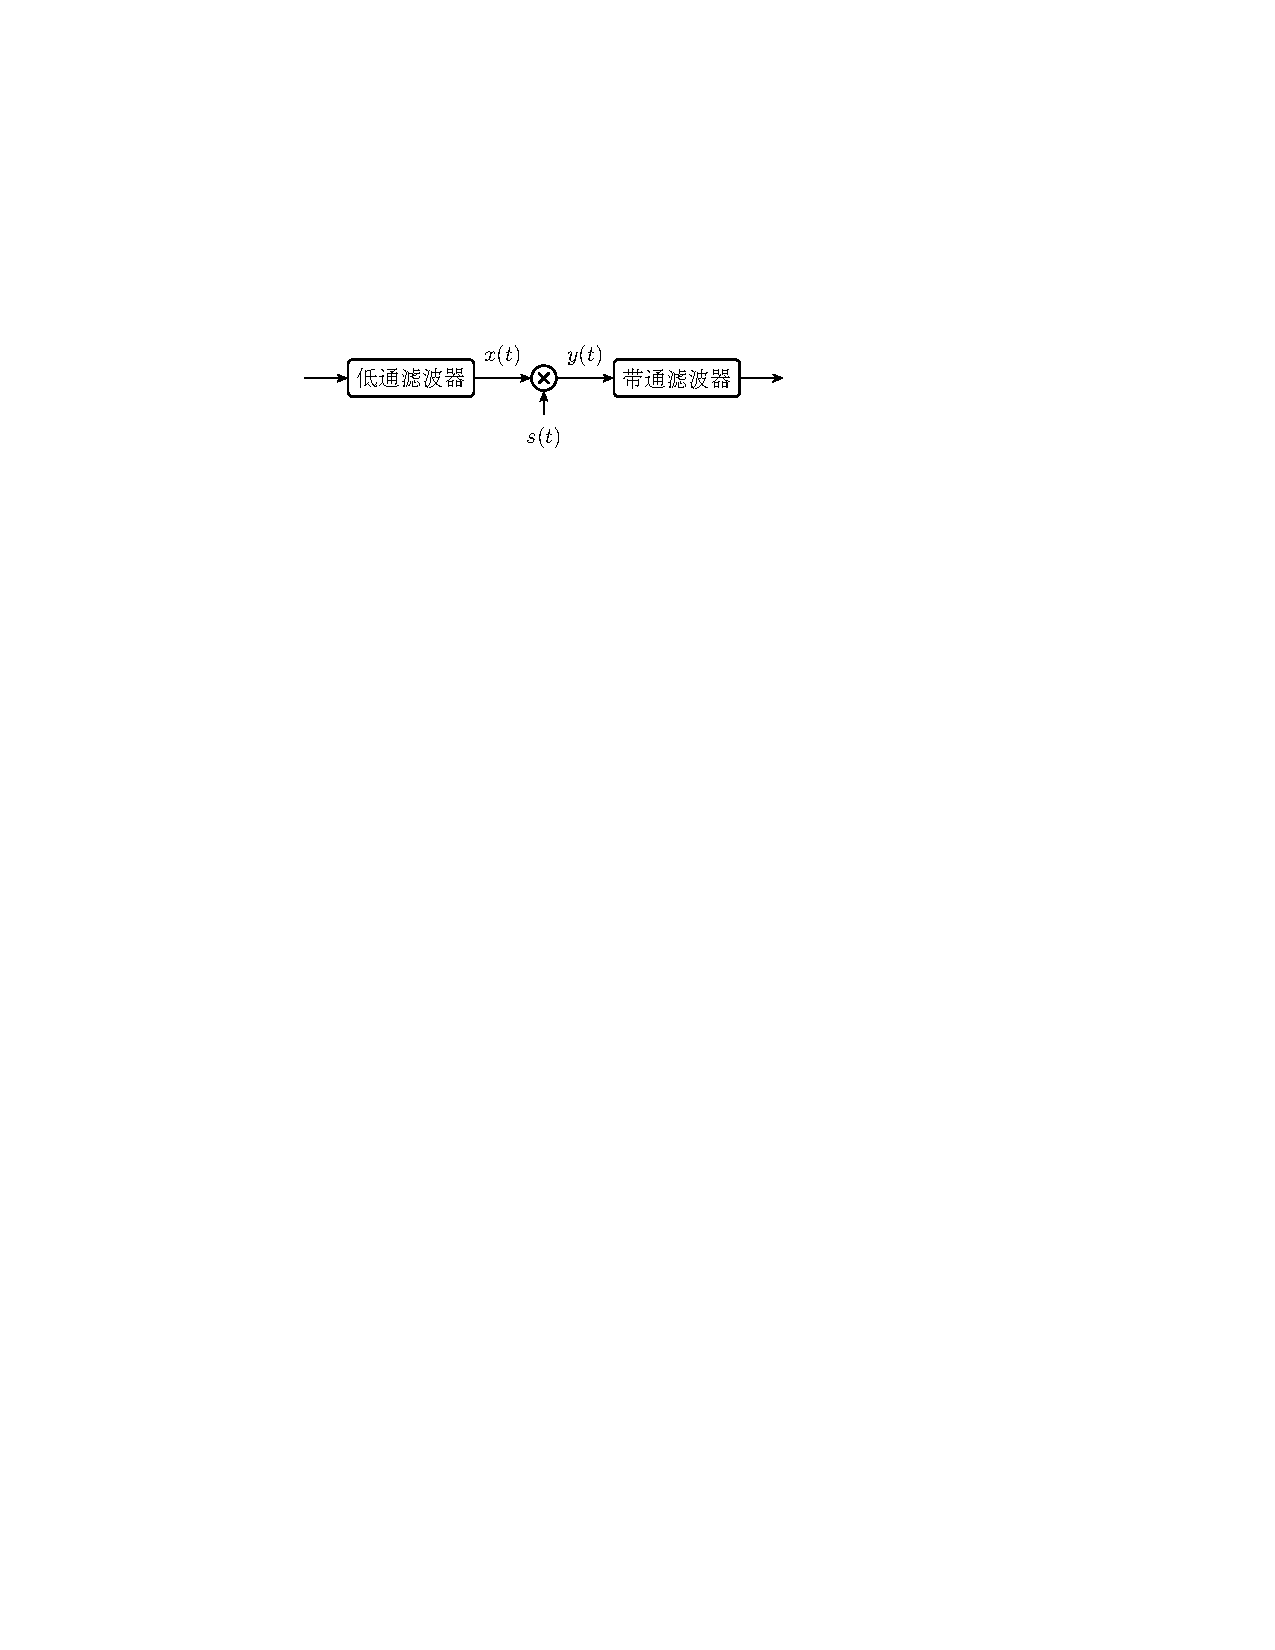
\includegraphics{img/5.pdf}\\
{\zihao{5}图4}
\end{center}
(1) 如图5所示系统,当输入为$f(t)=\dfrac{\sin(2\pi t)}{\pi t}$时,求通过理想滤波器$H_1(j\omega)$的输出信号$x(t)$;

(2) 已知$s(t)=\cos(6\pi t)$,要使$y(t)$通过融通滤波器$H_2(j\omega)$时能够完全通过,则此带通滤波器的最小带宽是多少?(也可以画图来说明)\par
\begin{center}
	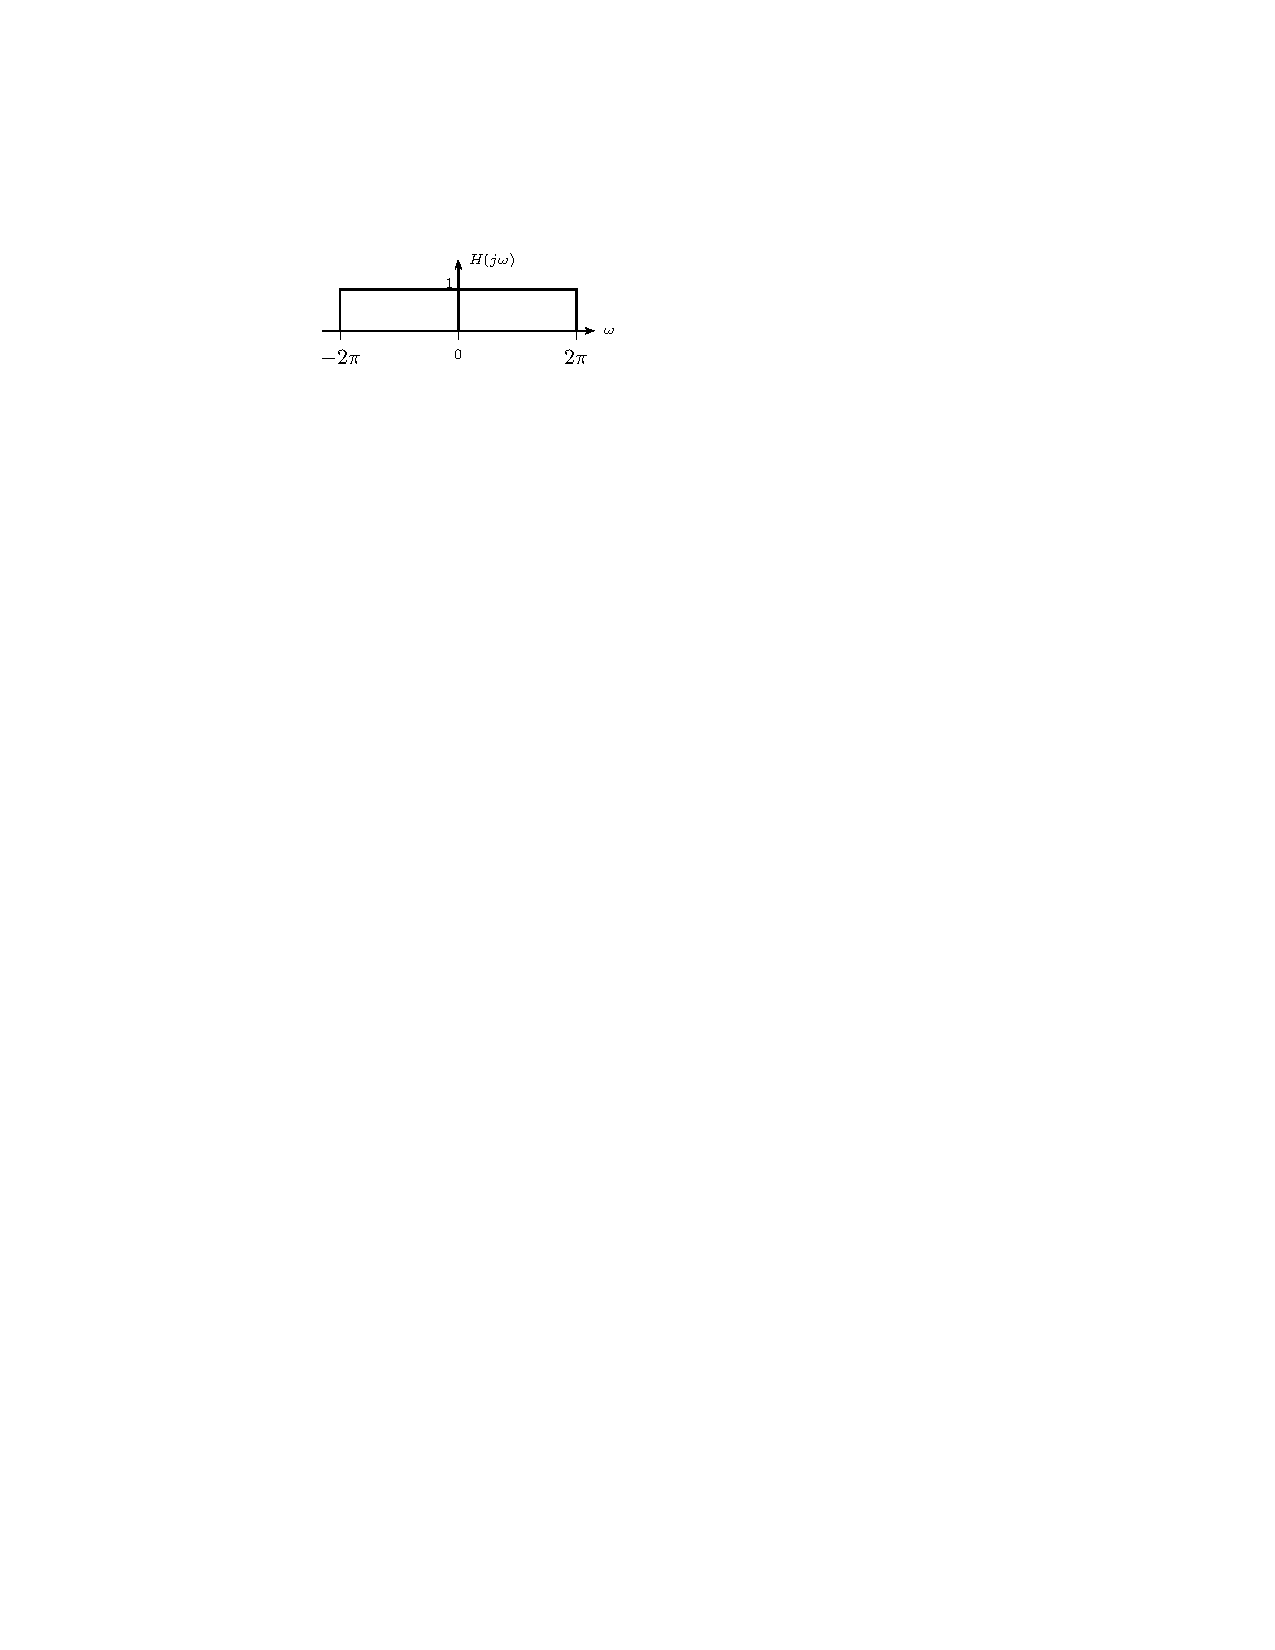
\includegraphics{img/14-2-3.pdf}\\
{\zihao{5}图5}
\end{center}
\vfill\newpage
%\item {\kaishu{}计算(每题4分)}\par
%\makebox[7.5cm][l]{(1)~$-17+(-16)-(-21)-13$}
%\makebox[7.5cm][l]{(2)~$-5m^2n-2mn+6nm^2-3mn$}
%\vfill
%\makebox[7.5cm][l]{(3)~$4y^2-[3y-(3-2y)+2y^2]$}
%\makebox[7.5cm][l]{(4)~$\left(\dfrac{2}{3}-\dfrac{1}{12}-\dfrac{4}{15}\right)\times(-60)$}
%% \vfill
%% \makebox[7.5cm][l]{\ding{176}~~$-2^2\div\dfrac{2}{3}-(-\dfrac{2}{3})\times(-30)$}
%\vfill
%\newpage
%
%	试卷背面
%
%\item (6分)先化简,再求值~.~其中$a=1$~.\\
%\makebox[10cm][c]{$\dfrac{1}{4}(-4a^2+2a-8)-2(\dfrac{1}{4}a-1)-1$}
%% \makebox[10cm][c]{$-2x^2+y^2-(2y^2-3x^2)+2(y^2-2x^2)$}
%\vfill
%% \item (7分)某城市出租车收费标准如下:3公里以内(含3公里)收费8元,超过3 公里的部分每公里收费1.5元.\\
%% (1)若行驶$x$公里($x$为整数),试用含$x$的代数式表示应收的车费;\\
%% (2)若某人乘坐出租汽车行驶8公里,则应付车费多少元?
%
%\item (8分)“十一”黄金周期间,某市风景区在7天假期中每天旅游的人数变化如下表(\uwave{正数表示比前一天多的人数,负数表示比前一天少的人数}):\par\hfill\null
%\begin{tabular}{|c|*{7}{|p{0.88cm}<{\centering}}|}
%\hline
%日期&1日&2日&3日&4日&5日&6日&7日\\\hline
%人数变化(单位:万人)&1.6&0.8&0.4&$-0.4$&$-0.8$&0.2&$-1.2$\\\hline
%\end{tabular}\hfill\null\par
%已知9月30日的游客人数为2万人,请回答下列问题:\\
%(1)七天内游客人数最多的是哪天,最少的是哪天?它们相差多少万人?\\
%%3.6,4.4,4.8,4.4,3.6,3.8,2.6
%(2)求这7天的游客总人数是多少万人.
%%27.2
%\vfill
%\item (7分)如图,在一个长方形休闲广场的四角都设计一块半径相同的四分之一圆形的花坛.若广场的长为$a$米,宽为$b$米,圆形的半径为$r$米~.~\\
%(1)~~请列式表示广场空地的面积;\\
%(2)~~若休闲广场的长为100米,宽为50米,圆形花坛的半径为10米,\\
%{\color{white}(1)}~~求广场空地的面积~.~(\uwave{计算结果保留$\pi$})\\
%\makebox[14cm][r]{\includegraphics[scale=0.55]{t23.png}}
%\vfill
%\newpage
%\item (4分)下图是由一些火柴棒搭成的图案,请观察图案并填表。\par\hfill\null
%\begin{tabular}{|c|*{6}{|p{1.2cm}<{\centering}}|}
%\hline
%五边形的个数&1&2&3&4&$\cdots$&$n$\\\hline
%火柴棒的根数&5&9~&~&~&$\cdots$&\\\hline
%\end{tabular}\hfill\null
%
%\hfill\null\makebox[13cm][c]{\includegraphics[scale=2]{t19.png}}\hfill\null
%
%% \vfill
%\item (6分)一种蔬菜$x$千克,不加工直接出售每千克可卖$y$元;如果经过加工重量减少了20\%,价格增加了40\%~.~问:
%$x$千克这种蔬菜加工后可卖多少钱?
%\vfill
%\item (8分)在一次抗震救灾中,某市组织20辆汽车装运食品、药品、生活用品三种救灾物资到灾民安置区,按计划每辆汽车只能装运一种救灾物资且必须装满~.~已知用了$a$辆汽车装运食品,用了$b$辆汽车装运药品,其余剩下的汽车装运生活用品,根据表中提供的信息,解答下列问题:\par\hfill
%\begin{tabular}{|c|*{3}{|p{2cm}<{\centering}}|}
%\hline
%物资种类&食品&药品&生活用品\\\hline
%每辆汽车运载(吨)&6&5&4\\\hline
%每吨所需运费(元)&120&160&100\\\hline
%\end{tabular}\hfill\null\par
%(1)20辆汽车共装载了多少吨救灾物资?\par
%(2)装运这批救灾物资的总费用是多少元?
%\vfill
% \newpage
\end{enumerate}
\end{document}
